\section{Clase 3}

\subsection{Técnicas de remuestreo}

En inferencia estadística interesa conocer cómo cambiaría un estimador si se
repitiera el proceso de muestreo. En la práctica, muchas veces solo se dispone
de una muestra. Las técnicas de remuestreo usan los datos observados para
construir muestras sintéticas y estudiar la variabilidad de los resultados.

Sea $\vec{x}=(x_1,\ldots,x_n)$ la muestra observada y $\theta$ el
parámetro de interés. Se usan minúsculas para los valores observados y
mayúsculas para variables aleatorias cuando es útil distinguirlas. El estimador
calculado con la muestra completa se denota por
\[
    \widehat\theta_n=T_n(\vec{x}),
\]
donde $T_n$ es el estadístico o regla de estimación. En esta clase se estudian
dos procedimientos: el \emph{jackknife}, que retira observaciones de manera
sistemática, y el \emph{bootstrap}, que vuelve a muestrear con reemplazo.
Ambos aproximan aspectos de la distribución muestral del estimador, pero
construyen las muestras sintéticas de manera distinta. La referencia anotada
en el cuaderno para estas técnicas es Feigelson.

\subsection{Jackknife: eliminar una observación}

\subsubsection{Muestras de eliminación individual}

El jackknife de eliminación individual (\emph{leave-one-out}) forma $n$
muestras, cada una con $n-1$ datos. La muestra $i$-ésima omite $x_i$ y conserva
todos los demás valores:
\[
    \vec{x}_{(-i)}=(x_1,\ldots,x_{i-1},x_{i+1},\ldots,x_n),
    \qquad i=1,\ldots,n.
\]
Al aplicar el mismo procedimiento de estimación a cada muestra reducida se
obtienen
\[
    \widehat\theta_{(-i)}=T_{n-1}(\vec{x}_{(-i)}),
    \qquad i=1,\ldots,n.
\]
La notación $(-i)$ indica que se excluyó la observación $i$; no significa que
se haya cambiado el valor de esa observación. Cada estimación permite ver qué
tanto depende el resultado de una observación particular.

\begin{figure}[htbp]
\centering
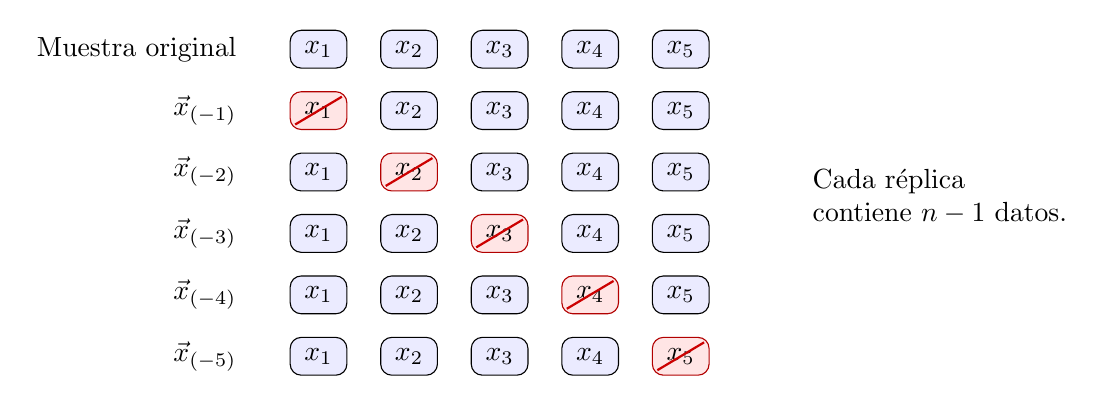
\begin{tikzpicture}[x=1.15cm,y=0.78cm,
  dato/.style={draw,rounded corners,minimum width=0.72cm,minimum height=0.48cm},
  omitido/.style={dato,fill=red!10,draw=red!70!black}]
  \node[anchor=east] at (-0.8,0) {Muestra original};
  \foreach \i in {1,...,5} {
    \pgfmathtruncatemacro{\pos}{\i-1}
    \node[dato,fill=blue!8] at (\pos,0) {$x_{\i}$};
  }
  \foreach \r in {1,...,5} {
    \pgfmathtruncatemacro{\y}{-\r}
    \node[anchor=east] at (-0.8,\y) {$\vec{x}_{(-\r)}$};
    \foreach \i in {1,...,5} {
      \pgfmathtruncatemacro{\pos}{\i-1}
      \ifnum\i=\r
        \node[omitido] (omit-\r) at (\pos,\y) {$x_{\i}$};
        \draw[red!80!black,thick] ([xshift=2pt,yshift=2pt]omit-\r.south west) -- ([xshift=-2pt,yshift=-2pt]omit-\r.north east);
      \else
        \node[dato,fill=blue!8] at (\pos,\y) {$x_{\i}$};
      \fi
    }
  }
  \node[anchor=west,align=left] at (5.35,-2.4)
    {Cada réplica\\ contiene $n-1$ datos.};
\end{tikzpicture}
\caption{Jackknife de eliminación individual para una muestra de tamaño cinco. En cada fila se excluye, por turno, una observación distinta.}
\label{fig:jackknife-muestras}
\end{figure}

\subsubsection{Promedio y corrección del sesgo}

El promedio de las estimaciones de eliminación individual es
\[
    \overline{\widehat\theta}_{(-\cdot)}
    =\frac{1}{n}\sum_{i=1}^{n}\widehat\theta_{(-i)}.
\]
El punto en el subíndice $(-\cdot)$ indica el promedio sobre el índice
$i=1,\ldots,n$ de la observación que se omite.

Se utiliza para estimar el sesgo del estimador de muestra completa. La
estimación jackknife del sesgo es
\[
    \widehat{\operatorname{bias}}_{J}(\widehat\theta_n)
    =(n-1)\left(
        \overline{\widehat\theta}_{(-\cdot)}-\widehat\theta_n
    \right)
    =\frac{n-1}{n}\sum_{i=1}^{n}
        \left(\widehat\theta_{(-i)}-\widehat\theta_n\right).
\]
El factor $n-1$ ajusta la diferencia entre el promedio de estimadores
calculados con $n-1$ datos y el estimador calculado con los $n$ datos
originales. Si el sesgo estimado es positivo, la corrección reduce la
estimación original; si es negativo, la aumenta. El estimador corregido es
\[
    \widehat\theta_{J,\mathrm{corr}}
    =\widehat\theta_n-
      \widehat{\operatorname{bias}}_{J}(\widehat\theta_n)
    =n\widehat\theta_n-(n-1)
      \overline{\widehat\theta}_{(-\cdot)}.
\]

\subsubsection{Pseudovalores}

También se puede escribir la corrección con los \emph{pseudovalores} del
jackknife:
\[
    P_i=n\widehat\theta_n-(n-1)\widehat\theta_{(-i)},
    \qquad i=1,\ldots,n.
\]
Su promedio es precisamente el estimador corregido:
\[
    \widehat\theta_{J,\mathrm{corr}}
    =\frac{1}{n}\sum_{i=1}^{n}P_i.
\]
Así, cada pseudovalor combina la estimación de la muestra completa con la
estimación que se obtuvo al quitar una observación. La figura resume el
proceso.

\begin{figure}[htbp]
\centering
\begin{tikzpicture}[
  caja/.style={draw,rounded corners,align=center,text width=3.0cm,minimum height=1.05cm},
  flecha/.style={-{Stealth[length=2.2mm]},thick}]
  \node[caja,fill=blue!7] (original) at (0,0)
    {Muestra completa\\$\widehat\theta_n$};
  \node[caja,fill=orange!10] (loo) at (4.3,0)
    {Réplicas jackknife\\$\widehat\theta_{(-1)},\ldots,\widehat\theta_{(-n)}$};
  \node[caja,fill=green!10] (pseudo) at (8.6,0)
    {Pseudovalores\\$P_i=n\widehat\theta_n-(n-1)\widehat\theta_{(-i)}$};
  \node[caja,fill=purple!9] (corrected) at (12.9,0)
    {Corrección\\$\widehat\theta_{J,\mathrm{corr}}=\dfrac{1}{n}\sum_{i=1}^{n}P_i$};
  \draw[flecha] (original) -- (loo);
  \draw[flecha] (loo) -- (pseudo);
  \draw[flecha] (pseudo) -- (corrected);
\end{tikzpicture}
\caption{De la muestra completa y las réplicas jackknife se construyen pseudovalores; su promedio es el estimador corregido.}
\label{fig:pseudovalores-jackknife}
\end{figure}

\subsubsection{Ejemplo: el jackknife para la media}

Considere la muestra $\{2,4,7,9\}$, de tamaño $n=4$. La media de la muestra
completa es $\widehat\theta_4=22/4=5.5$. Al retirar cada dato se obtiene:
\begin{center}
\begin{tabularx}{0.92\linewidth}{@{}cXcc@{}}
    \toprule
    $i$ & Muestra $\vec{x}_{(-i)}$ & $\widehat\theta_{(-i)}$ & $P_i$\\
    \midrule
    1 & $\{4,7,9\}$ & $20/3$ & $2$\\
    2 & $\{2,7,9\}$ & $6$ & $4$\\
    3 & $\{2,4,9\}$ & $5$ & $7$\\
    4 & $\{2,4,7\}$ & $13/3$ & $9$\\
    \bottomrule
\end{tabularx}
\end{center}
El promedio de las medias de eliminación es $\overline{\widehat\theta}_{(-\cdot)}=5.5$,
por lo que en este caso
\[
    \widehat{\operatorname{bias}}_{J}=3(5.5-5.5)=0,
    \qquad
    \widehat\theta_{J,\mathrm{corr}}=5.5.
\]
Los pseudovalores son los datos originales, $P_i=x_i$, y su promedio vuelve
a ser $5.5$. Para la media muestral, el jackknife no modifica la estimación:
la media de los promedios de eliminación individual coincide con la media de
la muestra completa.

\subsubsection{Variabilidad jackknife}

Además de corregir el sesgo, las réplicas jackknife permiten estimar la
varianza del estimador:
\[
    \widehat{\operatorname{Var}}_{J}(\widehat\theta_n)
    =\frac{n-1}{n}\sum_{i=1}^{n}
      \left(\widehat\theta_{(-i)}-
      \overline{\widehat\theta}_{(-\cdot)}\right)^2,
    \qquad
    \widehat{\operatorname{SE}}_{J}(\widehat\theta_n)
    =\sqrt{\widehat{\operatorname{Var}}_{J}(\widehat\theta_n)}.
\]
El error estándar resume la variación estimada del procedimiento de
estimación. Las $n$ réplicas jackknife no son muestras independientes: se
traslapan casi por completo, y la fórmula anterior tiene en cuenta esa
construcción.

\subsection{Bootstrap: muestrear con reemplazo}

\subsubsection{Distribución empírica y muestras bootstrap}

La distribución empírica de la muestra observada $\vec{x}$ es
\[
    \widehat F_n(t)=\frac{1}{n}\sum_{i=1}^{n}\mathbf 1(x_i\leq t).
\]
Asigna probabilidad $1/n$ a cada observación. Para construir la réplica
bootstrap $b$, se extraen $n$ valores independientemente de esta distribución,
condicionando en la muestra original:
\[
    X_{bj}^*\mid\vec{x}\overset{\mathrm{iid}}{\sim}\widehat F_n,
    \qquad j=1,\ldots,n,\quad b=1,\ldots,B.
\]
Aquí $B$ es el número de réplicas y
\[
    \vec{X}_b^*=(X_{b1}^*,\ldots,X_{bn}^*),
    \qquad \widehat\theta_b^*=T_n(\vec{X}_b^*),
    \qquad b=1,\ldots,B.
\]
El asterisco identifica cantidades bootstrap. Como el muestreo es con
reemplazo, una observación puede aparecer más de una vez y otra puede no
aparecer en una réplica. La muestra original se mantiene fija; se vuelve a
muestrear de $\widehat F_n$ para cada réplica.

\begin{figure}[htbp]
\centering
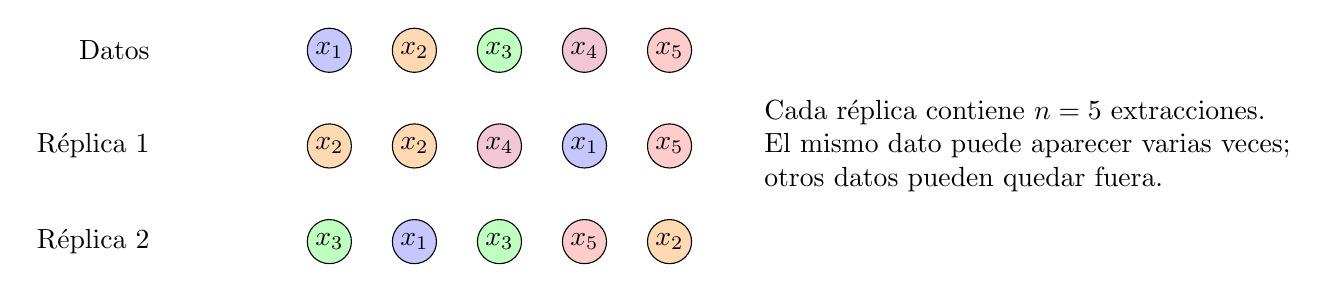
\begin{tikzpicture}[x=1.08cm,y=0.9cm,
  punto/.style={circle,draw,minimum size=0.56cm,inner sep=0pt},
  a/.style={punto,fill=blue!22}, b/.style={punto,fill=orange!30},
  c/.style={punto,fill=green!25}, d/.style={punto,fill=purple!22},
  e/.style={punto,fill=red!20}]
  \node[anchor=east] at (-1.0,0) {Datos};
  \foreach \i/\cl in {1/a,2/b,3/c,4/d,5/e}
    \node[\cl] at (\i,0) {$x_{\i}$};

  \node[anchor=east] at (-1.0,-1.35) {Réplica $1$};
  \foreach \j/\cl/\val in {1/b/2,2/b/2,3/d/4,4/a/1,5/e/5}
    \node[\cl] at (\j,-1.35) {$x_{\val}$};

  \node[anchor=east] at (-1.0,-2.7) {Réplica $2$};
  \foreach \j/\cl/\val in {1/c/3,2/a/1,3/c/3,4/e/5,5/b/2}
    \node[\cl] at (\j,-2.7) {$x_{\val}$};

  \node[anchor=west,align=left] at (6.0,-1.35)
    {Cada réplica contiene $n=5$ extracciones.\\El mismo dato puede aparecer varias veces;\\otros datos pueden quedar fuera.};
\end{tikzpicture}
\caption{Dos muestras bootstrap posibles extraídas con reemplazo de los cinco datos observados. El color identifica el dato de origen y permite ver las repeticiones.}
\label{fig:muestras-bootstrap}
\end{figure}

\subsubsection{Distribución empírica de las estimaciones}

Las estimaciones $\widehat\theta_1^*,\ldots,\widehat\theta_B^*$ forman una
distribución empírica en la escala del estimador. Para distinguirla de la
distribución empírica de los datos $\widehat F_n$, la denotamos por
\[
    \widehat F_{\mathrm{boot},B}(t)
    =\frac{1}{B}\sum_{b=1}^{B}
      \mathbf 1(\widehat\theta_b^*\leq t).
\]
Un histograma de estas estimaciones permite visualizar su centro y su
dispersión. Esta distribución aproxima la variabilidad del estimador bajo
remuestreo desde $\widehat F_n$; no es la distribución exacta del parámetro
ni reemplaza la distribución muestral teórica cuando esta se conoce.

\begin{figure}[htbp]
\centering
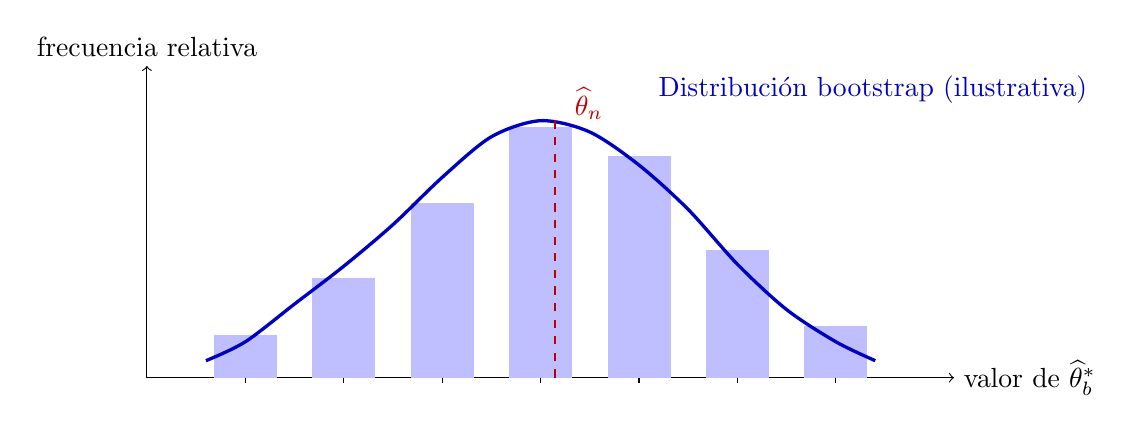
\begin{tikzpicture}[x=1.25cm,y=1.2cm]
  \draw[->] (0,0) -- (8.2,0) node[right] {valor de $\widehat\theta_b^*$};
  \draw[->] (0,0) -- (0,3.3) node[above] {frecuencia relativa};
  \foreach \x in {1,...,7}
    \draw (\x,0) -- (\x,-0.06);
  \foreach \x/\h in {1/0.45,2/1.05,3/1.85,4/2.65,5/2.35,6/1.35,7/0.55}
    \fill[blue!25] (\x-0.32,0) rectangle (\x+0.32,\h);
  \draw[very thick,blue!75!black] plot[smooth] coordinates {
    (0.6,0.18) (1,0.38) (1.5,0.78) (2,1.18) (2.5,1.62)
    (3,2.12) (3.5,2.55) (4,2.72) (4.5,2.60) (5,2.25)
    (5.5,1.78) (6,1.20) (6.5,0.72) (7,0.38) (7.4,0.18)
  };
  \draw[dashed,red!75!black,thick] (4.15,0) -- (4.15,2.8);
  \node[anchor=west,red!75!black] at (4.25,2.9) {$\widehat\theta_n$};
  \node[anchor=west,blue!75!black] at (5.1,3.05) {Distribución bootstrap (ilustrativa)};
\end{tikzpicture}
\caption{Distribución bootstrap ilustrativa de las estimaciones $\widehat\theta_b^*$. Su dispersión describe la variabilidad del estimador bajo remuestreo; la línea roja marca la estimación obtenida con la muestra original.}
\label{fig:distribucion-bootstrap}
\end{figure}

\subsubsection{Centro, sesgo y error estándar bootstrap}

El promedio de las estimaciones bootstrap es
\[
    \overline{\widehat\theta}^{\,*}_B
    =\frac{1}{B}\sum_{b=1}^{B}\widehat\theta_b^*.
\]
Este promedio estima el valor esperado del estimador bajo la distribución
empírica. A partir de las réplicas se estiman el sesgo y el error estándar:
\[
    \widehat{\operatorname{bias}}_{B}(\widehat\theta_n)
    =\overline{\widehat\theta}^{\,*}_B-\widehat\theta_n,
    \qquad
    \widehat{\operatorname{SE}}_{B}(\widehat\theta_n)
    =\sqrt{\frac{1}{B-1}\sum_{b=1}^{B}
      \left(\widehat\theta_b^*-
      \overline{\widehat\theta}^{\,*}_B\right)^2}.
\]
El estimador original $\widehat\theta_n$ sigue siendo el valor calculado con
los datos observados; $\overline{\widehat\theta}^{\,*}_B$ se usa para resumir
la distribución bootstrap y estimar el sesgo. En general, aumentar $B$
reduce el error Monte Carlo de estos resúmenes, aunque no agrega observaciones
nuevas a la muestra original.

\subsection{Comparación y recomendaciones}

\begin{center}
\begin{tabularx}{\linewidth}{@{}l>{\raggedright\arraybackslash}X>{\raggedright\arraybackslash}X@{}}
    \toprule
    & \textbf{Jackknife} & \textbf{Bootstrap}\\
    \midrule
    Cómo remuestrea & Omite una observación por réplica. & Selecciona $n$ datos con reemplazo por réplica.\\
    Número de réplicas & $n$ réplicas de eliminación individual. & $B$ réplicas, que se eligen suficientemente numerosas para estabilizar los resultados.\\
    Uso principal & Diagnosticar influencia y aproximar sesgo y variabilidad. & Aproximar la distribución del estimador, su sesgo y su error estándar.\\
    Dependencia & Las réplicas se traslapan. & Las réplicas son aleatorias condicionadas a la muestra observada.\\
    \bottomrule
\end{tabularx}
\end{center}

En ambos métodos, las conclusiones dependen de que la muestra observada sea
razonablemente representativa y de que el estadístico se comporte de forma
regular ante pequeñas perturbaciones. El remuestreo cuantifica incertidumbre
a partir de los datos disponibles, pero no corrige por sí solo sesgos de
selección, datos faltantes ni errores del modelo.

\subsection{Resumen}

El jackknife construye $n$ estimaciones omitiendo un dato cada vez y usa sus
diferencias respecto de $\widehat\theta_n$ para estimar y corregir el sesgo.
Los pseudovalores permiten expresar el estimador corregido como un promedio.
El bootstrap genera $B$ nuevas muestras de tamaño $n$ con reemplazo desde la
distribución empírica y estudia la distribución de las estimaciones
resultantes. La distinción clave es: jackknife elimina datos de manera
sistemática; bootstrap vuelve a seleccionar datos aleatoriamente y puede
repetirlos.

\subsection{Ejercicio integrador resuelto}

\subsubsection*{Enunciado}

Considere la muestra observada $\vec{x}=(2,4,6,8)$ y use la media muestral
como estimador de $\theta$. Aplique los dos métodos de remuestreo vistos en
esta clase:
\begin{enumerate}
    \item Calcule la media de la muestra y las cuatro estimaciones jackknife
    de eliminación individual.
    \item Calcule el promedio de las estimaciones jackknife, el sesgo
    estimado, la corrección jackknife y los pseudovalores.
    \item Obtenga la varianza y el error estándar jackknife.
    \item Use las siguientes cuatro réplicas bootstrap, generadas con
    reemplazo, para calcular sus medias, el sesgo bootstrap y su error
    estándar:
    \[
        (2,4,4,8),\quad (2,2,6,8),\quad (4,6,6,8),\quad (2,4,6,8).
    \]
    \item Escriba la distribución empírica de las cuatro medias bootstrap y
    explique brevemente por qué los errores estándar jackknife y bootstrap
    pueden ser diferentes.
\end{enumerate}

\subsubsection*{Solución}

\begin{enumerate}
    \item La media de la muestra completa es
    \[
        \widehat\theta_4=\frac{2+4+6+8}{4}=5.
    \]
    Al omitir cada observación, las medias son
    \[
        \widehat\theta_{(-1)}=6,\qquad
        \widehat\theta_{(-2)}=\frac{16}{3},\qquad
        \widehat\theta_{(-3)}=\frac{14}{3},\qquad
        \widehat\theta_{(-4)}=4.
    \]

    \item El promedio jackknife coincide con la media original:
    $\overline{\widehat\theta}_{(-\cdot)}=5$. Así, el sesgo estimado es
    $3(5-5)=0$ y la estimación corregida sigue siendo $5$. Los pseudovalores
    son
    \[
        P_i=4(5)-3\widehat\theta_{(-i)},
        \qquad (P_1,P_2,P_3,P_4)=(2,4,6,8),
    \]
    y su promedio también es $5$.

    \item Aplicando la fórmula jackknife,
    \[
        \widehat{\operatorname{Var}}_J(\widehat\theta_4)
        =\frac{3}{4}\left[(6-5)^2+
          \left(\frac{16}{3}-5\right)^2+
          \left(\frac{14}{3}-5\right)^2+(4-5)^2\right]
        =\frac{5}{3}.
    \]
    Por tanto, $\widehat{\operatorname{SE}}_J=\sqrt{5/3}\approx1.291$.

    \item Las medias bootstrap son $4.5,\ 4.5,\ 6$ y $5$. Su promedio vale
    $5$, por lo que el sesgo estimado es $5-\widehat\theta_4=0$. El error
    estándar bootstrap es
    \[
        \widehat{\operatorname{SE}}_B
        =\sqrt{\frac{(4.5-5)^2+(4.5-5)^2+(6-5)^2+(5-5)^2}{3}}
        =\sqrt{0.5}\approx0.707.
    \]

    \item La distribución empírica de esas medias es
    \[
        \widehat F_{\mathrm{boot},4}(t)=
        \begin{cases}
            0, & t<4.5,\\
            1/2, & 4.5\leq t<5,\\
            3/4, & 5\leq t<6,\\
            1, & t\geq6.
        \end{cases}
    \]
    Los errores estándar pueden diferir porque resumen conjuntos de réplicas
    construidos de maneras distintas. Además, con solo cuatro réplicas
    bootstrap, el resultado es ilustrativo y puede cambiar al generar más.
\end{enumerate}
La figura compara visualmente las estimaciones de ambos procedimientos con la
media obtenida de la muestra completa.
\begin{figure}[htbp]
\centering
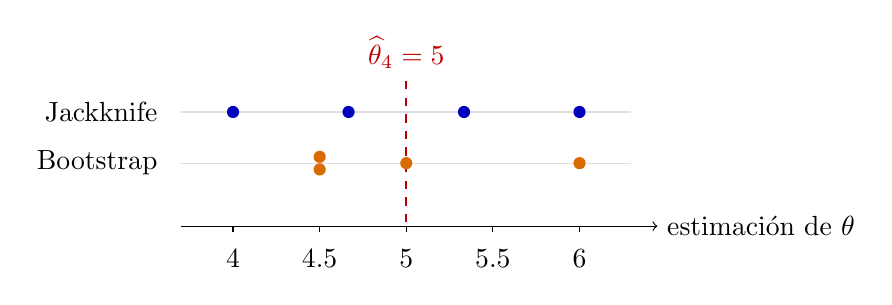
\begin{tikzpicture}[x=2.2cm,y=1cm]
  \draw[gray!25] (3.7,1.45) -- (6.3,1.45);
  \draw[gray!25] (3.7,0.8) -- (6.3,0.8);
  \draw[->] (3.7,0) -- (6.45,0)
    node[right] {estimación de $\theta$};
  \foreach \x/\lab in {4/4,4.5/4.5,5/5,5.5/5.5,6/6} {
    \draw (\x,0) -- (\x,-0.07) node[below=3pt] {$\lab$};
  }
  \node[anchor=east] at (3.62,1.45) {Jackknife};
  \node[anchor=east] at (3.62,0.8) {Bootstrap};
  \draw[dashed,red!75!black,thick] (5,0.05) -- (5,1.88);
  \node[above,red!75!black] at (5,1.88) {$\widehat\theta_4=5$};

  \foreach \x in {4,4.6667,5.3333,6}
    \fill[blue!75!black] (\x,1.45) circle (2.2pt);

  \fill[orange!85!black] (4.5,0.72) circle (2.2pt);
  \fill[orange!85!black] (4.5,0.88) circle (2.2pt);
  \fill[orange!85!black] (5,0.8) circle (2.2pt);
  \fill[orange!85!black] (6,0.8) circle (2.2pt);
\end{tikzpicture}
\caption{Estimaciones de eliminación jackknife y medias de las cuatro réplicas bootstrap del ejercicio. Los dos puntos apilados en $4.5$ corresponden a dos réplicas con la misma media; la línea roja señala la media de la muestra completa.}
\label{fig:integrador-clase3}
\end{figure}